\documentclass[a4paper,14pt]{article}
\usepackage[a4paper, mag=1000, left=2.5cm, right=1cm, top=2cm, bottom=2cm, headsep=0.7cm, footskip=1cm]{geometry}
\usepackage[utf8]{inputenc}
\usepackage[T2A]{fontenc}
\usepackage[english,russian]{babel}
\usepackage{indentfirst}
%\usepackage[dvipsnames]{xcolor}
%\usepackage[colorlinks]{hyperref}
\usepackage{amsfonts} 
\usepackage{amsmath}
\usepackage{graphicx}
\usepackage{float}

\DeclareGraphicsExtensions{.png,.jpg}

\usepackage{fancyhdr}
\pagestyle{fancy}
\fancyhead[LE,RO]{\thepage}
\fancyfoot{}

\usepackage{listings}

%\hypersetup{linkcolor=black}

\title{non-linear equations}
\author{Иван Золин}
\date{2023}
\thispagestyle{empty}
\begin{document}
	
	\begin{titlepage}
		\begin{center}
			\textsc{
				Санкт-Петербургский политехнический университет имени Петра Великого \\[5mm]
				Институт прикладной математики и механики\\[2mm]
				Высшая школа прикладной математики и физики            
			}   
			\vfill
			\textbf{\large
				Математическая статистика\\
				Отчёт по лабораторным работам №1-4 \\[3mm]
			}                
		\end{center}
		
		\vfill
		\hfill
		\begin{minipage}{0.5\textwidth}
			Выполнил: \\[2mm]   
			Студент: Макарова Арина \\
			Группа: 5030102/00101\\
		\end{minipage}
		
		\hfill
		\begin{minipage}{0.5\textwidth}
			Принял: \\[2mm]
			к. ф.-м. н., доцент \\   
			Баженов Александр Николаевич
		\end{minipage}
		
		\vfill
		\begin{center}
			Санкт-Петербург \\2023 г.
		\end{center}
	\end{titlepage}
	
	\tableofcontents
	\newpage
	\listoffigures
	\newpage
	\listoftables
	\newpage
	
	\section{Постановка задачи}
	\paragraph{Для четырех распределений:}
	\begin{itemize}
		\item Нормальное распределение: $N(x, 0, 1)$
		\item Распределение Коши: $C(x, 0, 1)$
		\item Распределение Лапласа: $L(x, 0, \frac{1}{\sqrt{2}})$
		\item Распределение Пуассона: $P(k, 10)$
		\item Равномерное распределение: $U(x, -\sqrt{3}, \sqrt{3})$
	\end{itemize}
	\paragraph{Выполнить следующие задачи:}
	\begin{enumerate}
		\item Сгенерировать выборки размером 10, 50 и 1000 элементов.
		Построить на одном рисунке гистограмму и график плотности распределения.
		
		\item Сгенерировать выборки размером 10, 100 и 1000 элементов.
		Для каждой выборки вычислить следующие статистические характеристики положения данных: $\overline{x}, med x, z_R, z_Q, z_{tr}$. Повторить такие вычисления 1000 раз для каждой выборки и найти среднее характеристик положения и их квадратов:
		
		\begin{equation}
			E(z)=\overline{z}
		\end{equation}
		
		Вычислить оценку дисперсии по формуле:
		
		\begin{equation}
			D(z)=\overline{z^2}-\overline{z}^2
		\end{equation}
		
		Представить полученные данные в виде таблиц.
		
		\item Сгенерировать выборки размером 20 и 100 элементов.
		\newline Построить для них боксплот Тьюки.
		Для каждого распределения определить долю выбросов экспериментально (сгенерировав выборку, соответствующую распределению 1000
		раз, и вычислив среднюю долю выбросов) и сравнить с результатами,
		полученными теоретически.
		
		\item Сгенерировать выборки размером 20, 60 и 100 элементов.
		Построить на них эмпирические функции распределения и ядерные оценки плотности распределения на отрезке $[-4; 4]$ для непрерывных распределений и на отрезке $[6; 14]$ для распределения Пуассона.
	\end{enumerate}
	\newpage
	\section{Теория}
	\subsection{Распределения}
	Плотности классических распределений:
	
	\begin{itemize}
		\item Нормальное распределение
		
		\begin{equation}
			N(x, 0, 1) = \tfrac{1}{\sqrt{2\pi}}e^{-\frac{x^2}{2}}
		\end{equation}
		
		\item Распределение Коши
		
		\begin{equation}
			C(x, 0, 1) = \dfrac{1}{\pi}\dfrac{1}{x^2+1}
		\end{equation}
		
		\item Распределение Лапласа
		
		\begin{equation}
			L(x, 0, \frac{1}{\sqrt{2}}) =\frac{1}{\sqrt{2}}e^{-{\sqrt{2}}|x|}
		\end{equation}
		
		\item Распределение Пуассона
		
		\begin{equation}
			P(k, 10) = \tfrac{10^k}{k!}e^{-10}
		\end{equation}
		
		\item Равномерное распределение
		
		\begin{equation}
			U(x, -\sqrt{3}, \sqrt{3}) =
			\begin{cases} 
				\;\; \dfrac{1}{2\sqrt{3}} \;\;\;\; \text{при} \;\;\;\; |x| \leq \sqrt{3}\\
				\,\,\,\:\;\; 0 \;\;\;\;\;\;\; \text{при} \;\;\;\; |x| > \sqrt{3}
			\end{cases}
		\end{equation}
		
	\end{itemize}
	
	\subsubsection{Определение}
	
	Гистограмма в математической статистике --- это функция, приближающая плотность вероятности некоторого распределения, построенная на основе выборки из него \cite{s:hist}.
	
	\subsubsection{Графическое описание}
	
	Графически гистограмма строится следующим образом. Сначала множество значений, которое может принимать элемент выборки, разбивается на несколько интервалов. Чаще всего эти интервалы берут одинаковыми, но это не является строгим требованием. Эти интервалы откладываются на горизонтальной оси, затем над каждым рисуется прямоугольник. Если все интервалы были одинаковыми, то высота каждого прямоугольника пропорциональна числу элементов выборки, попадающих в соответствующий интервал. Если интервалы разные, то высота прямоугольника выбирается таким образом, чтобы его площадь была пропорциональна числу элементов выборки, которые попали в этот интервал \cite{s:hist}.
	
	\subsubsection{Использование}
	
	Гистограммы применяются в основном для визуализации данных на начальном этапе статистической обработки.\\
	Построение гистограмм используется для получения эмпирической оценки плотности распределения случайной величины. Для построения гистограммы наблюдаемый диапазон изменения случайной величины разбивается на несколько интервалов и подсчитывается доля от всех измерений, попавшая в каждый из интервалов. Величина каждой доли, отнесенная к величине интервала, принимается в качестве оценки значения плотности распределения на соответствующем интервале \cite{s:hist}.\\
	Они являются мощным инструментом для исследования неизвестных распределений.\\
	В частности, на этом построены различные способы обработки сигналов, изображений и других статистических объектов. Применение гистограмм к обработке экспериментальных данных позволяет устранять артефакты - шумы и выбросы, мешающие работе с данными и не являющиеся содержательными. \\
	Шумы определяются как горизонтальные участки сигнала. Присутствуют они только до и
	после полезного сигнала, на нем они быть не могут. Определяются участки шума так: находятся границы 2-ух самых больших столбцов гистограммы полученного сигнала, затем путем прохода по сигналу в обе стороны окном определнного размера и сравнения процентного соотношения значений внутри границ большого столбца с выбранным порогом, принимается решение о пометке участка как шумового при превышении этого порога.\\
	Выбросы —  экстремальные значения во входных данных, находящиеся далеко за пределами других наблюдений. На гистограмме выбросы будут формировать одиночные пики. Выбросы следует заменить чем-то разумным (средним, медианой в окрестности). Нужно идти по гистограмме скользящим окном (параметр), и, что вылетает далеко по гистограмме (или за 3 сигмы), заменять медианным значением. Тогда ожидается, что колонны гистограммы сравняются с пейзажем.
	
	
	\subsection{Вариационный ряд}
	
	Вариационным рядом называется последовательность элементов выборки, расположенных в неубывающем порядке. Одинаковые элементы повторяются \cite[с. 409]{b:probSectMath}.\\
	Запись вариационного ряда: $x_{(1)}, x_{(2)}, \, ... \: , x_{(n)}$.\\
	Элементы вариационного ряда $x_{(i)} \;\; (i = 1, 2, \, ... \: , n)$ называются порядковыми статистиками.
	
	\subsection{Выборочные числовые характеристики}
	
	С помощью выборки образуются её числовые характеристики. Это числовые характеристики дискретной случайной величины $X^*$, принимающей выборочные значения $x_1, x_2, \, ... \: , x_n$ \cite[с. 411]{b:probSectMath}.
	
	\subsubsection{Характеристики положения}
	
	\begin{itemize}
		\item Выборочное среднее
		
		\begin{equation} \label{eq:mean}
			\overline{x} = \tfrac{1}{n}\sum\limits_{i=1}^n x_i
		\end{equation}
		
		\item Выборочная медиана
		
		\begin{equation} \label{eq:med}
			med \: x = 
			\begin{cases} 
				\;\;\;\;\;\;\; x_{(l+1)} \:\;\;\;\;\;\;\;\;\; \text{при} \;\;\;\; n = 2l + 1\\
				\;\; \dfrac{x_{(l)} + x_{(l+1)}}{2} \;\;\;\; \text{при} \;\;\;\; n = 2l
			\end{cases}
		\end{equation}
		
		\item Полусумма экстремальных выборочных элементов
		
		\begin{equation} \label{eq:zR}
			z_R = \dfrac{x_{(1)} + x_{(n)}}{2}
		\end{equation}
		
		\item Полусумма квартилей
		
		Выборочная квартиль $z_p$ порядка $p$ определяется формулой
		
		\begin{equation}
			z_p =
			\begin{cases}
				\;\; x_{([np]+1)} \;\;\;\; \text{при} \;\; np \;\; \text{дробном},\\
				\;\;\;\;\; x_{(np)} \,\:\;\;\;\;\; \text{при} \;\; np \;\; \text{целом}.
			\end{cases}
		\end{equation}
		
		Полусумма квартилей
		
		\begin{equation} \label{eq:zQ}
			z_Q = \dfrac{z_{1/4} + z_{3/4}}{2}
		\end{equation}
		
		\item Усечённое среднее
		
		\begin{equation} \label{eq:zTr}
			z_{tr} = \tfrac{1}{n-2r}\sum\limits_{i=r+1}^{n-r} x_{(i)}, \;\;\;\; r \approx \dfrac{n}{4}
		\end{equation}
		
	\end{itemize}
	
	\subsubsection{Характеристики рассеяния}
	
	Выборочная дисперсия
	
	\begin{equation}
		D = \tfrac{1}{n}\sum\limits_{i=1}^{n} (x_i - \overline{x})^2
	\end{equation}
	
	\subsection{Боксплот Тьюки}
	
	\subsubsection{Определение}
	
	Боксплот (англ. box plot) --- график, использующийся в описательной статистике, компактно изображающий одномерное распределение вероятностей.
	
	\subsubsection{Описание}
	
	Такой вид диаграммы в удобной форме показывает медиану, нижний и верхний квартили и выбросы. Несколько таких ящиков можно нарисовать бок о бок, чтобы визуально сравнивать одно распределение с другим; их можно располагать как горизонтально, так и вертикально. Расстояния между различными частями ящика позволяют определить степень разброса (дисперсии) и асимметрии данных и выявить выбросы \cite{s:boxplot}. 
	
	\subsubsection{Построение}
	
	Границами ящика служат первый и третий квартили, линия в середине ящика --- медиана. Концы усов --- края статистически значимой выборки (без выбросов). Длину «усов» определяют разность первого квартиля и полутора межквартильных расстояний и сумма третьего квартиля и полутора межквартильных расстояний. Формула имеет вид
	
	\begin{equation} \label{eq:boundBoxplot}
		X_1 = Q_1 - \dfrac{3}{2}(Q_3 - Q_1), \;\; X_2 = Q_3 + \dfrac{3}{2}(Q_3 - Q_1),
	\end{equation}
	
	где $X_1$ --- нижняя граница уса, $X_2$ --- верхняя граница уса, $Q_1$ --- первый квартиль, $Q_3$ --- третий квартиль.
	
	Данные, выходящие за границы усов (выбросы), отображаются на графике в виде маленьких кружков \cite{s:boxplot}.
	
	\subsection{Теоретическая вероятность выбросов}
	
	Встроенными средствами языка программирования R в среде разработки RStudio можно вычислить теоретические первый и третий квартили распределений ($Q_1^\text{т}$ и $Q_3^\text{т}$ соответственно). По формуле \eqref{eq:boundBoxplot} можно вычислить теоретические нижнюю и верхнюю границы уса ($X_1^\text{т}$ и $X_2^\text{т}$ соответственно). Выбросами считаются величины $x$, такие что:
	
	\begin{equation}
		\left[ 
		\begin{gathered} 
			x < X_1^\text{т}\\ 
			x > X_2^\text{т}\\ 
		\end{gathered} 
		\right.
	\end{equation}
	
	Теоретическая вероятность выбросов для непрерывных распределений
	
	\begin{equation} \label{eq:probTheorCont}
		P_\text{в}^\text{т} = P(x < X_1^\text{т}) + P(x > X_2^\text{т}) = F(X_1^\text{т}) + \Big(1 - F(X_2^\text{т})\Big),
	\end{equation}
	
	где $F(X) = P(x \le X)$ - функция распределения.\\
	
	Теоретическая вероятность выбросов для дискретных распределений
	
	\begin{equation} \label{eq:probTheorDisc}
		P_\text{в}^\text{т} = P(x < X_1^\text{т}) + P(x > X_2^\text{т}) = \Big(F(X_1^\text{т}) - P(x = X_1^\text{т})\Big) + \Big(1 - F(X_2^\text{т})\Big),
	\end{equation}
	
	где $F(X) = P(x \le X)$ - функция распределения.
	
	\subsection{Эмпирическая функция распределения}
	
	\subsubsection{Статистический ряд}
	
	Статистическим рядом называется последовательность различных элементов выборки $z_1, z_2, \, ... \: , z_k$, расположенных в возрастающем порядке с указанием частот $n_1, n_2, \, ... \: , n_k$, с которыми эти элементы содержатся в выборке.
	
	Статистический ряд обычно записывается в виде таблицы
	
	\begin{table}[h!]
		\begin{center}
			\begin{tabular}{|c|c|c|c|c|}
				\hline
				$z$ & $z_1$ & $z_2$ & $...$ & $z_k$ \\
				\hline
				$n$ & $n_1$ & $n_2$ & $...$ & $n_k$ \\
				\hline
			\end{tabular}
		\end{center}
		\caption{Статистический ряд}
	\end{table} 
	
	\subsubsection{Определение}
	
	Эмпирической (выборочной) функцией распределения (э. ф. р.) называется относительная частота события $X < x$, полученная по данной выборке:
	
	\begin{equation}
		F_n^*(x) = P^*(X < x).
	\end{equation}
	
	\subsubsection{Описание}
	
	Для получения относительной частоты $P^*(X < x)$ просуммируем в статистическом ряде, построенном по данной выборке, все частоты $n_i$, для которых элементы $z_i$ статистического ряда меньше $x$. Тогда $P^*(X < x) = \tfrac{1}{n}\sum\limits_{z_i < x}n_i$. Получаем
	
	\begin{equation}
		F^*(x) = \tfrac{1}{n}\sum\limits_{z_i < x}n_i.
	\end{equation}
	
	$F^*(x)$ --- функция распределения дискретной случайной величины $X^*$, заданной таблицей распределения
	
	\begin{table}[h!]
		\begin{center}
			\begin{tabular}{|c|c|c|c|c|}
				\hline
				$X^*$ & $z_1$ & $z_2$ & $...$ & $z_k$ \\
				\hline
				$P$ & $\dfrac{n_1}{n}$ & $\dfrac{n_2}{n}$ & $...$ & $\dfrac{n_k}{n}$ \\
				\hline
			\end{tabular}
		\end{center}
		\caption{Таблица распределения}
	\end{table}
	
	Эмпирическая функция распределения является оценкой, т. е. приближённым значением, генеральной функции распределения
	
	\begin{equation}
		F_n^*(x) \approx F_X(x).
	\end{equation}
	
	\subsection{Оценки плотности вероятности}
	
	\subsubsection{Определение}
	
	Оценкой плотности вероятности $f(x)$ называется функция $\widehat{f}(x)$, построенная на основе выборки, приближённо равная $f(x)$
	
	\begin{equation}
		\widehat{f}(x) \approx f(x).
	\end{equation}
	
	\subsubsection{Ядерные оценки}
	
	Представим оценку в виде суммы с числом слагаемых, равным объёму выборки:
	
	\begin{equation}
		\widehat{f}_n(x) = \tfrac{1}{nh_n}\sum\limits_{i=1}^n K\left( \tfrac{x - x_i}{h_n} \right).
	\end{equation}
	
	Здесь функция $K(u)$, называемая ядерной (ядром), непрерывна и является плотностью вероятности, $x_1, \, ... \: , x_n$ --- элементы выборки, $\{h_n\}$ --- любая последовательность положительных чисел, обладающая свойствами
	
	\begin{equation}
		h_n \underset{n \to \infty}{\longrightarrow} 0; \qquad \dfrac{h_n}{n^{-1}} \underset{n \to \infty}{\longrightarrow} \infty.
	\end{equation}
	
	Такие оценки называются непрерывными ядерными \cite[с. 421-423]{b:probSectMath}.\\
	
	Замечание. Свойство, означающее сближение оценки с оцениваемой величиной при $n \rightarrow \infty$ в каком-либо смысле, называется состоятельностью оценки.\\
	
	Если плотность $f(x)$ кусочно-непрерывная, то ядерная оценка плотности является состоятельной при соблюдении условий, накладываемых на параметр сглаживания $h_n$, а также на ядро $K(u)$.\\
	
	Гауссово (нормальное) ядро \cite[с. 38]{a:nonParamRegr}
	
	\begin{equation}
		K(u) = \tfrac{1}{\sqrt{2\pi}}e^{-\tfrac{u^2}{2}}.
	\end{equation}
	
	Правило Сильвермана \cite[с. 44]{a:nonParamRegr}
	
	\begin{equation}
		h_n = 1.06\hat{\sigma}n^{-1/5},
	\end{equation}
	
	где $\hat{\sigma}$ - выборочное стандартное отклонение.
	
	\subsubsection{Оценка качества ядерных приближений}
	
	После получения результатов возникает необходимость оценить качество ядерных приближений. Приведем в пример один из приемов количественных описаний сходства кривых - метод Фреше. \\
	
	Расстояние Фреше $-$ это мера сходства кривых, принимающая во внимание число и порядок точек вдоль кривых. Расстояние названо по имени французского математика Мориса Фреше.
	Метрика Фреше принимает во внимание течение лвух кривых, посколько пары точек, расстояние между которыми определяет расстояние Фреше, <<пробегают>> вдоль кривых.
	Расстояние Фреше между двумя кривыми $-$ это не длина самого короткого поводка, с котрым можно пройти все пути, а самый короткий, при котором можно пройти этот путь. \\
	
	Определим кривую как непрерывное отображение $f: [a,b] \rightarrow V$, где $a, b \in R$ и $a \leq b$ и $(V,d) - $ метрическое пространство.
	Даны две кривые $f: [a,b] \rightarrow V$ и $g: [a',b'] \rightarrow V$, их расстояние Фреше определено в виде:
	\begin{equation}
		\delta F(f,g) = \inf_{\alpha, \beta}\max_{t \in [0,1]}{\{d(f(\alpha(t)), g(\beta(t)))\}}
	\end{equation}
	
	где $\alpha$ (соответственно $\beta$) $-$ произвольная непрерывная неубывающая функция из $[0, 1]$ на $[a, b]$ (соттветственно $[a',b']$). \\
	При вычислении расстояния Фреше между произвольными кривыми обычно аппроксимируют кривые многоугольными кривыми. Многоульная кривая $-$ это кривая $P: [0,n] \rightarrow V$, где $n - $ натуральное число, такое, что для каждого $i \in [0,n-1]$ ограничение $P$ к интервалу $[i,i+1]$ является аффинным, то есть $P(i+\lambda) = (1-\lambda)P(i)+\lambda P(i+1)$. \\
	Для заданных многоугольных кривых $P$ и $Q$ их дискретное расстояние Фреше определяется как:
	%\begin{equation}
	%\delta_{dF}(P,Q)=min\norm L \norm
	%\end{equation}
	где $L - PQ$.
	
	Необязательно решение $ - $ пара точек, между которыми найдено расстояние Фреше, $-$ является единственным. \\
	
	Рассмотрим расстояние Фреше для двух кривых: ядерной оценки плотности для равномерного распределения и самого равномерного распределения при $n=100$:
		\section{Реализация}
	\subsection{Описание}
	Данная лабораторная работа была выполнена с использованием языка
	программирования R в среде разработки RStudio и Python 3.8 в среде разработки VSCode с
	использованием следующих библиотек:
	\begin{itemize}
		\item math - использование математических функций
		\item matplotlib версии 3.7.1 - построение графиков
		\item numpy версии 1.24.2 - использование многомерных массивов
		\item prettytable версии 3.6.0 - вывод таблиц в консоли 
		\item scipy версии 1.10.1 - статические распределения и функции
		\item seaborn версии 0.12.2 - посроение графиков, визуализация
		\item statsmodels - дополнение к scipy, использование статистических вычислений, включая описательную статистику, оценку и вывод статистических моделей
	\end{itemize}
	Отчёт подготовлен с помощью языка LaTEX в редакторе TexStudio.
		\subsection{Ссылка на репозиторий}
		\url{https://github.com/ArinaMak/Mathematical-statistics/tree/main/labs/lab1} \ - GitHub репозиторий
	
	\section{Результаты}
	\subsection{Гистограмма и график плотности распределения}
	\begin{figure}[H]
		\centering
		\begin{tabular}{c c c}
			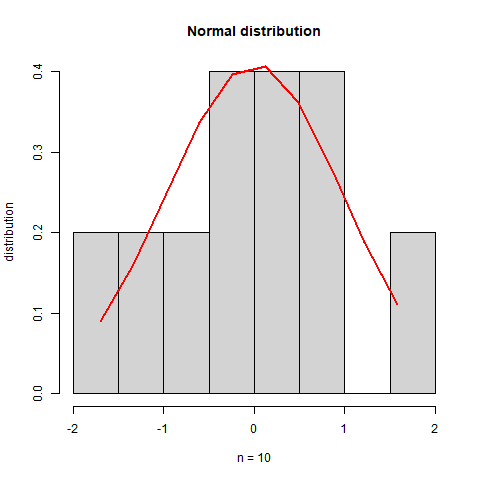
\includegraphics[height = 0.25\textheight, width = 0.31\textwidth]{./lab1_1/pictures/ n = 10 normal distribution.png}
			& 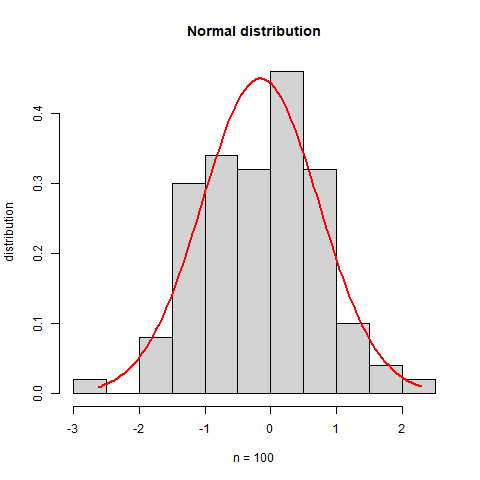
\includegraphics[height = 0.25\textheight, width = 0.31\textwidth]{./lab1_1/pictures/ n = 100 normal distribution.png}
			& 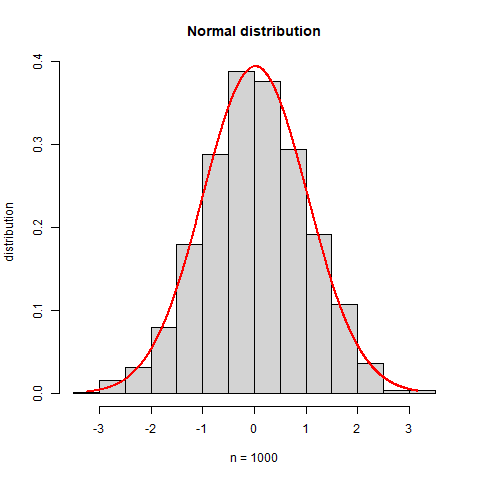
\includegraphics[height = 0.25\textheight, width = 0.31\textwidth]{./lab1_1/pictures/ n = 1000 normal distribution.png}
		\end{tabular}
		\caption{Нормальное распределение}
	\end{figure}
	
	\begin{figure}[H]
		\centering
		\begin{tabular}{c c c}
			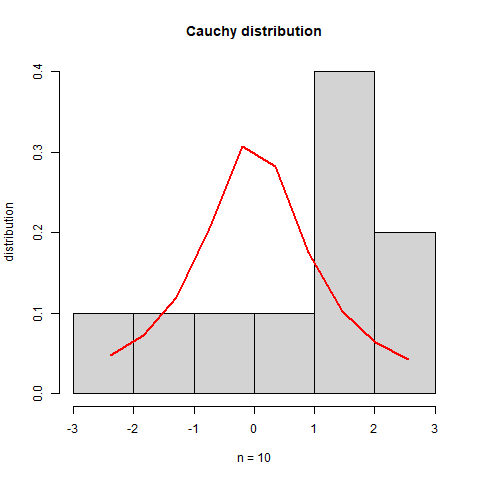
\includegraphics[height = 0.25\textheight, width = 0.31\textwidth]{./lab1_1/pictures/ n = 10 cauchy distribution.png}
			& 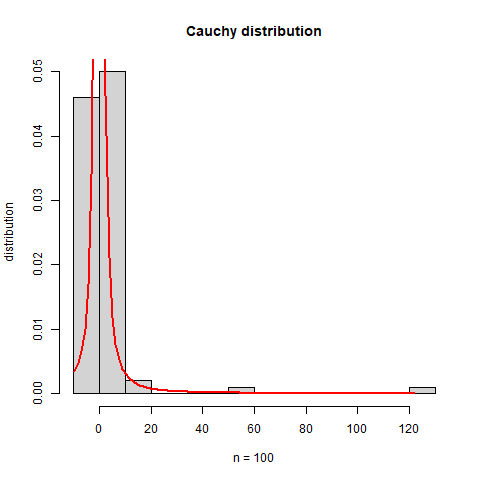
\includegraphics[height = 0.25\textheight, width = 0.31\textwidth]{./lab1_1/pictures/ n = 100 cauchy distribution.png}
			& 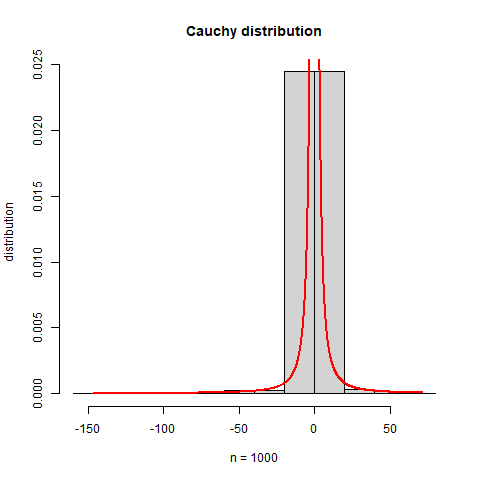
\includegraphics[height = 0.25\textheight, width = 0.31\textwidth]{./lab1_1/pictures/ n = 1000 cauchy distribution.png}
		\end{tabular}
		\caption{Распределение Коши}
	\end{figure}
	
	\begin{figure}[H]
		\centering
		\begin{tabular}{c c c}
			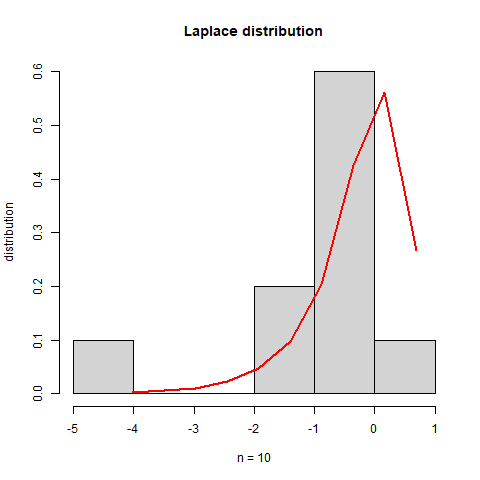
\includegraphics[height = 0.25\textheight, width = 0.31\textwidth]{./lab1_1/pictures/ n = 10 laplace distribution.png}
			& 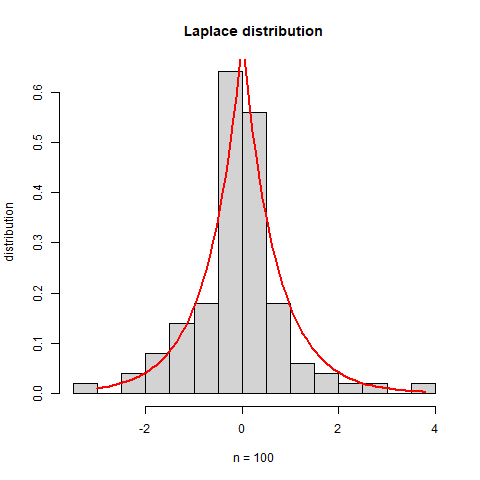
\includegraphics[height = 0.25\textheight, width = 0.31\textwidth]{./lab1_1/pictures/ n = 100 laplace distribution.png}
			& 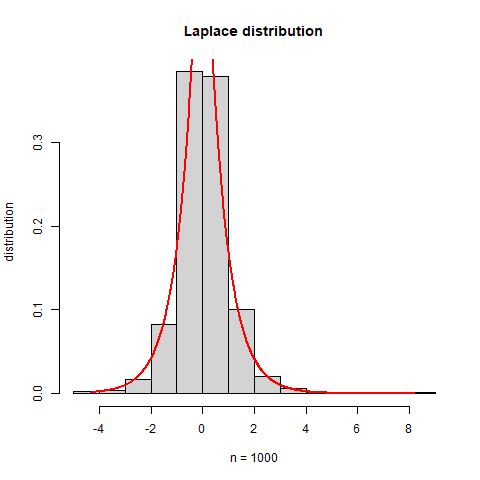
\includegraphics[height = 0.25\textheight, width = 0.31\textwidth]{./lab1_1/pictures/ n = 1000 laplace distribution.png}
		\end{tabular}
		\caption{Распределение Лапласа}
	\end{figure}
	
	\begin{figure}[H]
		\centering
		\begin{tabular}{c c c}
			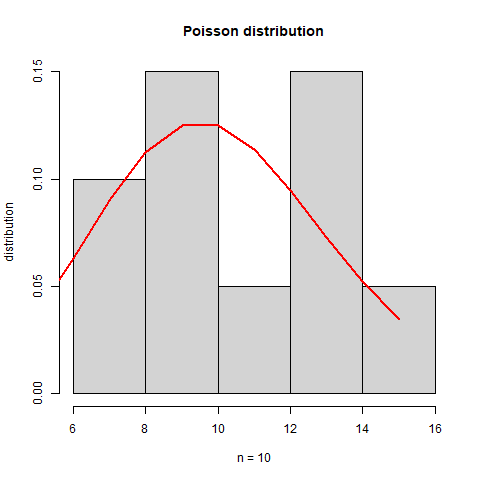
\includegraphics[height = 0.25\textheight, width = 0.31\textwidth]{./lab1_1/pictures/ n = 10 poisson distribution.png}
			& 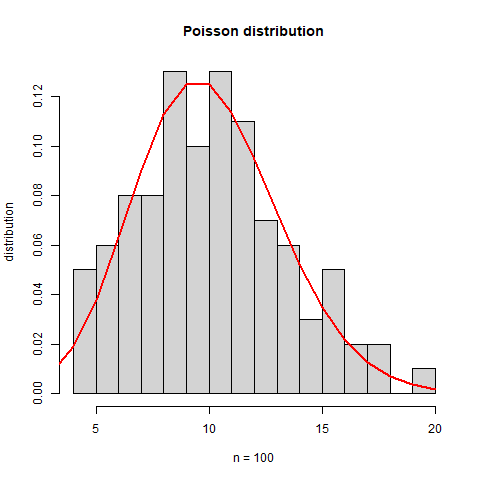
\includegraphics[height = 0.25\textheight, width = 0.31\textwidth]{./lab1_1/pictures/ n = 100 poisson distribution.png}
			& 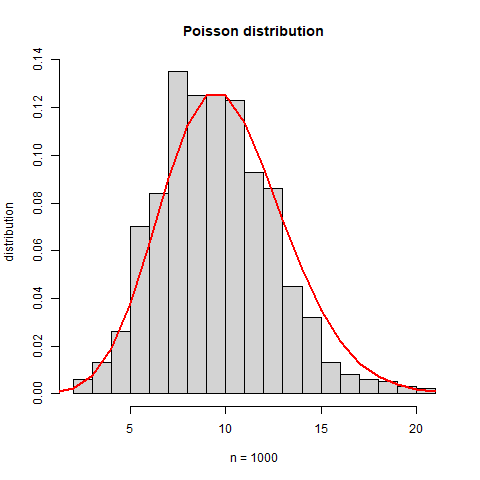
\includegraphics[height = 0.25\textheight, width = 0.31\textwidth]{./lab1_1/pictures/ n = 1000 poisson distribution.png}
		\end{tabular}
		\caption{Распределение Пуассона}
	\end{figure}
	
	\begin{figure}[H]
		\centering
		\begin{tabular}{c c c}
			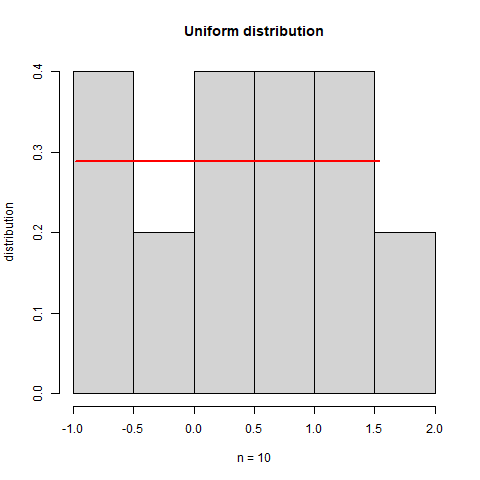
\includegraphics[height = 0.25\textheight, width = 0.31\textwidth]{./lab1_1/pictures/ n = 10 uniform distribution.png}
			& 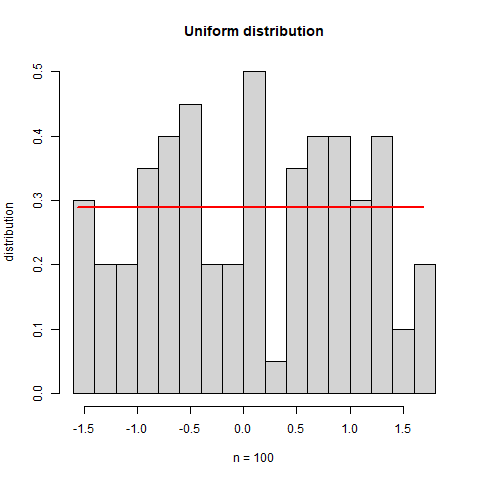
\includegraphics[height = 0.25\textheight, width = 0.31\textwidth]{./lab1_1/pictures/ n = 100 uniform distribution.png}
			& 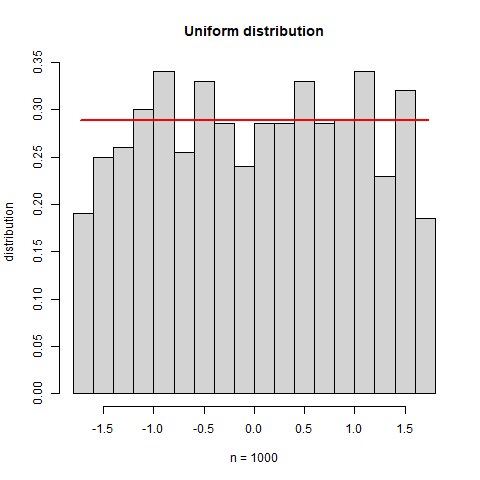
\includegraphics[height = 0.25\textheight, width = 0.31\textwidth]{./lab1_1/pictures/ n = 1000 uniform distribution.png}
		\end{tabular}
		\caption{Равномерное распределение}
	\end{figure}
	\subsection{Характеристики положения и рассеяния}
	Как было проведено округление:\\
	В оценке $x=E  \pm D$ вариации подлежит первая цифра после точки. \\
	В данном случае $x=0.0 \pm 0.1k$,\\
	$k$ - зависит от доверительной вероятности и вида распределения (рассматривается в дальнейшем цикле лабораторных работ). \\
	Округление сделано для  $k=1$.
	
	\begin{table}[H]
		\centering
		\begin{tabular}[t]{|l|r|r|r|r|r|}
			\hline
			& $\overline{x}$ & $med x$ & $z_R$ & $z_Q$ & $z_{tr}$\\\hline\hline
			n=10 & & & & &\\\hline
			$E(z)$ & 0.0024 & -0.0029 & 0.016 & -0.0017 & -0.0053\\\hline
			$D(z)$ & 0.1029 & 0.143 & 0.180 & 0.123 & 0.117\\\hline
			$E(z)\pm\sqrt{D(z)}$ & [-0.32;0.32] & [-0.38;0.38] & [-0.41;0.44] & [-0.35;0.35] & [-0.35;0.34]\\\hline
			$\hat{E(z)}$ & 0 & 0 & 0 & 0 & 0\\\hline
			
			n=100 & & & & &\\\hline
			$E(z)$ & -0.0005 & 0.0018 & -0.019 & -0.0146 & 0.0018\\\hline
			$D(z)$ & 0.0106 & 0.016 & 0.097 & 0.013 & 0.012\\\hline
			$E(z)\pm\sqrt{D(z)}$ & [-0.1;0.1] & [-0.12;0.13] & [-0.33;0.29] & [-0.1;0.1] & [-0.1;0.1]\\\hline
			$\hat{E(z)}$ & 0 & 0 & 0 & 0 & 0\\\hline
			n=1000 & & & & &\\\hline
			$E(z)$ & -0.0004 & 0.0005 & -0.003 & -0.0023 & -0.0006\\\hline
			$D(z)$ & 0.0009 & 0.001 & 0.061 & 0.001 & 0.001\\\hline
			$E(z)\pm\sqrt{D(z)}$ & [-0.03;0.03] & [-0.03;0.04] & [-0.25;0.24] & [-0.03;0.03] & [-0.03;0.03]\\\hline
			$\hat{E(z)}$ & 0.0 & 0.0 & 0 & 0.0 & 0.0\\\hline

		\end{tabular}
		\caption{Таблица характеристик для нормального распределения}
		\label{tab:normal}
	\end{table}
	
	\begin{table}[H]
		\centering
		\begin{tabular}[t]{|l|r|r|r|r|r|}
			\hline
			& $\overline{x}$ & $med x$ & $z_R$ & $z_Q$ & $z_{tr}$\\\hline\hline
			n=10 & & & & &\\\hline
			$E(z)$  & -0.35 & 0.0155 & -1.647 & -0.0144 & 0.0027  \\\hline
$E(z)$  & 812.5582 & 0.3563 & 20102.12 & 1.1678 & 0.5375  \\\hline
$E(z)\pm\sqrt{D(z)}$  & [-28.9;28.2] & [-0.5814;0.6124] & [-143.4;140.1] & [ -1.095;1.0662 ] & [ -0.7304;0.7358 ]  \\\hline
			$\hat{E(z)}$ & - & 0 & - & - & 0\\\hline
			
			n=100 & & & & &\\\hline
			$E(z)$  & 4.9454 & -0.0003 & 251.956 & -0.0327 & 0.0003  \\\hline
$E(z)$  & 32298.13 & 0.0261 & 80527322 & 0.0513 & 0.0261  \\\hline
$E(z)\pm\sqrt{D(z)}$  & [ -174.8;184.7 ] & [ -0.1619;0.1613 ] & [ -8721.7;9225.7 ] & [ -0.2592;0.1938 ] & [ -0.1613;0.1619 ]  \\\hline
			$\hat{E(z)}$ & - & 0 & - & 0 & 0\\\hline
			
			n=1000 & & & & &\\\hline
			$E(z)$  & 1.1833 & -0.0013 & 611.3653 & -0.0055 & -0.0018  \\\hline
$E(z)$  & 16553.72 & 0.0025 & 4132734206 & 0.0051 & 0.0026  \\\hline
$E(z)\pm\sqrt{D(z)}$  & [ -127.5;129.8 ] & [ -0.0513;0.0487 ] & [ -63674.9;64897.7 ] & [ -0.0769;0.0659 ] & [ -0.0528;0.0492 ]  \\\hline
			$\hat{E(z)}$ & - & 0.0 & - & 0.0 & 0.0\\\hline
			
		\end{tabular}
		\caption{Таблица характеристик для распределения Коши}
		\label{tab:cauchy}
	\end{table}
	
	\begin{table}[H]
		\centering
		\begin{tabular}[t]{|l|r|r|r|r|r|}
			\hline
			& $\overline{x}$ & $med x$ & $z_R$ & $z_Q$ & $z_{tr}$\\\hline\hline
			n=10 & & & & &\\\hline
			$E(z)$  & -0.0163 & -0.0114 & -0.0234 & -0.0169 & -0.0139  \\\hline
$E(z)$  & 0.1003 & 0.0731 & 0.3897 & 0.1025 & 0.0753  \\\hline
$E(z)\pm\sqrt{D(z)}$  & [ -0.333;0.3004 ] & [ -0.2818;0.259 ] & [ -0.6477;0.6009 ] & [ -0.3371;0.3033 ] & [ -0.2883;0.2605 ]  \\\hline
			$\hat{E(z)}$ & 0 & 0 & 0 & 0 & 0\\\hline
			
			n=100 & & & & &\\\hline
			$E(z)$  & -0.0005 & 0.0014 & -0.0163 & -0.0158 & 0.0012  \\\hline
$E(z)$  & 0.0099 & 0.006 & 0.4152 & 0.0097 & 0.0062  \\\hline
$E(z)\pm\sqrt{D(z)}$  & [ -0.1;0.099 ] & [ -0.0761;0.0789 ] & [ -0.6607;0.6281 ] & [ -0.1143;0.0827 ] & [ -0.0775;0.0799 ]  \\\hline
			$\hat{E(z)}$ & 0 & 0.0 & 0 & 0 & 0.0\\\hline
			
			n=1000 & & & & &\\\hline
			$E(z)$  & 0.0004 & 0.0006 & -0.0025 & -0.0017 & 0.0005  \\\hline
$E(z)$  & 0.001 & 0.0005 & 0.4035 & 0.001 & 0.0006  \\\hline
$E(z)\pm\sqrt{D(z)}$  & [ -0.0312;0.032 ] & [ -0.0218;0.023 ] & [ -0.6377;0.6327 ] & [ -0.0333;0.0299 ] & [ -0.024;0.025 ]  \\\hline
			$\hat{E(z)}$ & 0.0 & 0.0 & 0 & 0.0 & 0.0\\\hline
			
		\end{tabular}
		\caption{Таблица характеристик для распределения Лапласа}
		\label{tab:laplace}
	\end{table}
	
	\begin{table}[H]
		\centering
		\begin{tabular}[t]{|l|r|r|r|r|r|}
			\hline
			& $\overline{x}$ & $med x$ & $z_R$ & $z_Q$ & $z_{tr}$\\\hline\hline
			n=10 & & & & &\\\hline
			$E(z)$  & 9.99 & 9.836 & 10.321 & 9.9375 & 9.8798  \\\hline
$E(z)$  & 1.03 & 1.4581 & 1.926 & 1.2318 & 1.162  \\\hline
$E(z)\pm\sqrt{D(z)}$  & [ 8.98; 11.01 ] & [ 8.62; 11.04 ] & [ 8.93; 11.71 ] & [ 8.83; 11.05 ] & [ 8.80; 10.96 ]  \\\hline
			$\hat{E(z)}$ & - & - & - & - & -\\\hline
			
			n=100 & & & & &\\\hline
			$E(z)$  & 9.99 & 9.8315 & 10.96 & 9.872 & 9.8523  \\\hline
$E(z)$  & 0.10 & 0.2134 & 0.9694 & 0.1611 & 0.1226  \\\hline
$E(z)\pm\sqrt{D(z)}$  & [ 9.68; 10.32 ] & [ 9.37; 10.29 ] & [ 9.98; 11.94 ] & [ 9.47; 10.27 ] & [ 9.50; 10.20 ]  \\\hline
			$\hat{E(z)}$ & - & - & - & - & -\\\hline
			
			n=1000 & & & & &\\\hline
			$E(z)$  & 9.99 & 9.9945 & 11.674 & 9.996 & 9.8579  \\\hline
$E(z)$  & 0.0098 & 0.0052 & 0.7037 & 0.002 & 0.0114  \\\hline
$E(z)\pm\sqrt{D(z)}$  & [ 9.90; 10.1 ] & [ 9.92; 10.07 ] & [ 10.84; 12.51 ] & [ 9.95; 10.04 ] & [ 9.75; 9.96 ]  \\\hline
			$\hat{E(z)}$ & - & - & - & - & -\\\hline
			
		\end{tabular}
		\caption{Таблица характеристик для распределения Пуассона}
		\label{tab:poisson}
	\end{table}
	
	\begin{table}[H]
		\centering
		\begin{tabular}[t]{|l|r|r|r|r|r|}
			\hline
			& $\overline{x}$ & $med x$ & $z_R$ & $z_Q$ & $z_{tr}$\\\hline\hline
			n=10 & & & & &\\\hline
			$E(z)$  & -0.0098 & -0.0208 & -0.0093 & -0.0007 & -0.0093  \\\hline
$E(z)$  & 0.3122 & 0.6971 & 0.1337 & 0.4298 & 0.5011  \\\hline
$E(z)\pm\sqrt{D(z)}$  & [ -0.57 ; 0.55 ] & [ -0.86 ; 0.81 ] & [ -0.38 ; 0.36 ] & [ -0.66 ; 0.65 ] & [ -0.72 ; 0.7 ]  \\\hline
			$\hat{E(z)}$ & 0 & 0 & 0 & 0 & 0\\\hline
			
			n=100 & & & & &\\\hline
			$E(z)$  & 0.0089 & 0.0145 & -0.002 & -0.0196 & 0.0138  \\\hline
$E(z)$  & 0.0288 & 0.0822 & 0.0019 & 0.0432 & 0.0566  \\\hline
$E(z)\pm\sqrt{D(z)}$  & [ -0.16 ; 0.18 ] & [ -0.27 ; 0.30 ] & [ -0.05 ; 0.04 ] & [ -0.23 ; 0.19 ] & [ -0.22 ; 0.25 ]  \\\hline
			$\hat{E(z)}$ & 0 & 0 & 0.0 & 0 & 0\\\hline
			
			n=1000 & & & & &\\\hline
			$E(z)$  & -0.0004 & -0.0035 & 0.0001 & -0.0026 & -0.0013  \\\hline
$E(z)$  & 0.003 & 0.0092 & 0 & 0.0045 & 0.0061  \\\hline
$E(z)\pm\sqrt{D(z)}$  & [ -0.06 ; 0.05 ] & [ -0.09 ; 0.09 ] & [ 0.0001 ; 0.0001 ] & [ -0.0697 ; 0.0645 ] & [ -0.0794 ; 0.0768 ]  \\\hline
			$\hat{E(z)}$ & 0.0 & 0.0 & 0.000 & 0.0 & 0.0\\\hline
			
		\end{tabular}
		\caption{Таблица характеристик для равномерного распределения}
		\label{tab:uniform}
	\end{table}
	\subsection{Боксплот Тьюки}
	\begin{figure}[H]
		\centering
		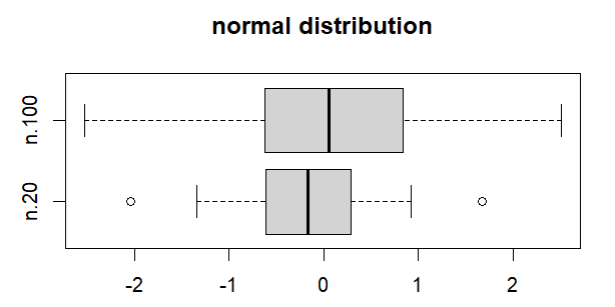
\includegraphics[scale=0.9]{./lab1_3/pictures/boxplot rnorm.PNG}
		\caption{Нормальное распределение}
		\label{fig:normal}
	\end{figure}
	
	\begin{figure}[H]
		\centering
		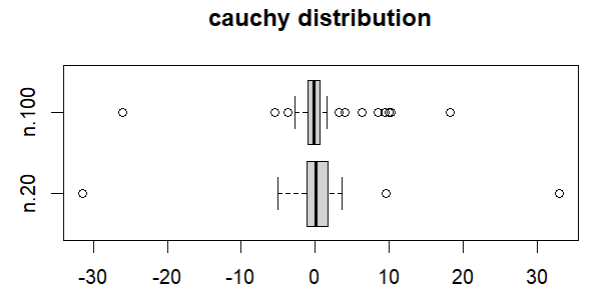
\includegraphics[scale=0.9]{./lab1_3/pictures/boxplot rcauchy.PNG}
		\caption{Распределение Коши}
		\label{fig:cauchy}
	\end{figure}
	
	\begin{figure}[H]
		\centering
		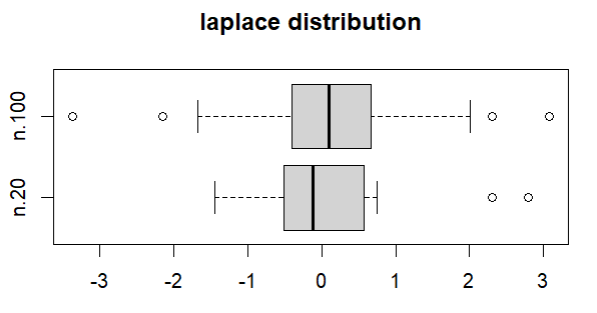
\includegraphics[scale=0.9]{./lab1_3/pictures/boxplot rlaplace.PNG}
		\caption{Распределение Лапласа}
		\label{fig:laplace}
	\end{figure}
	
	\begin{figure}[H]
		\centering
		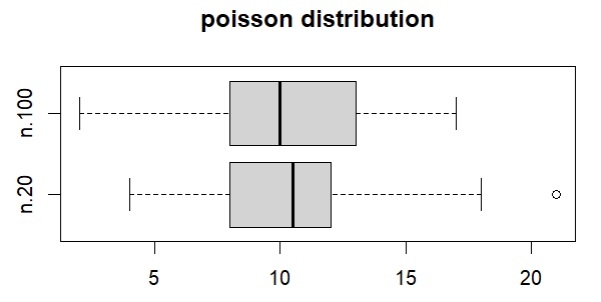
\includegraphics[scale=0.9]{./lab1_3/pictures/boxplot rpois.PNG}
		\caption{Распределение Пуассона}
		\label{fig:poisson}
	\end{figure}
	
	\begin{figure}[H]
		\centering
		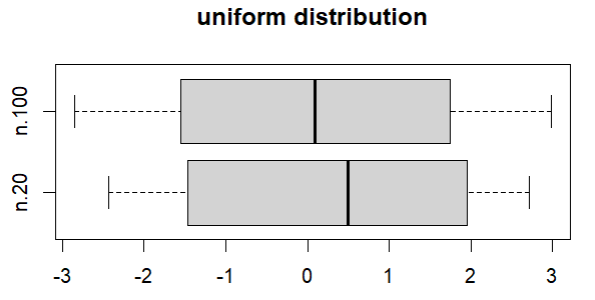
\includegraphics[scale=0.9]{./lab1_3/pictures/boxplot runif.PNG}
		\caption{Равномерное распределение}
		\label{fig:uniform}
	\end{figure}
	\subsection{Доля выбросов}
	Выборка случайна, поэтому в качестве оценки рассеяния можно взять дисперсию пуассоновского потока:  $D_n \approx \sqrt{n}$\\
	Доля $p_n = \frac{D_n}{n}=\frac{1}{\sqrt{n}}$\\
	Доля $n=20: p_n=\frac{1}{\sqrt{20}}$ - примерно 0.2 или 20\% \\
	Для $n=100: p_n=\frac{1}{\sqrt{100}}$ - примерно 0.1 или 10\% \\
	Исходя из этого можно решить, сколько знаков оставлять в доле выброса.
	
	\begin{table}[H]
		\centering
		\begin{tabular}{|l|c|c|}
			\hline
			Выборка & Доля выбросов	\\\hline
			\hline
			Normal n = 20 & 0.02 \\\hline
			Normal n = 100 & 0.01 \\\hline
			Cauchy n = 20 & 0.15 \\\hline
			Cauchy n = 100 & 0.16\\\hline
			Laplace n = 20 & 0.07 \\\hline
			Laplace n = 100 & 0.07 \\\hline
			Poisson n = 20 & 0.02 \\\hline
			Poisson n = 100 & 0.01 \\\hline
			Uniform n = 20 & 0.00 \\\hline
			Uniform n = 100 & 0.00 \\\hline
		\end{tabular}
		\caption{Практическая доля выбросов}
	\end{table}
	\subsection{Теоретическая вероятность выбросов}
	\begin{table}[H]
		\centering
		\begin{tabular}{|l|c|c|c|c|c|}
			\hline
			Распределение & $Q_1^T$	& $Q_3^T$ & $X_1^T$ & $X_2^T$ & $P_B^T$\\\hline
			\hline
			Нормальное & -0.672 & 0.669 & -2.685 & 2.682 & 0.007\\\hline
			Коши & -1.011 & 0.995 & -4.019 & 4.004 & 0.156\\\hline
			Лапласа & -0.490 & 0.487 & -1.956 & 1.952 & 0.063\\\hline
			Пуассона & 7.806 & 12.01 & 1.499 & 18.317 & 0.008\\\hline
			Равномерное & -0.844 & 0.850 & -3.386 & 3.392 & 0\\\hline
		\end{tabular}
		\caption{Теоретическая вероятность выбросов}
	\end{table}
	
	\subsection{Эмпирическая функция распределения}
	\begin{figure}[H]
		\centering
		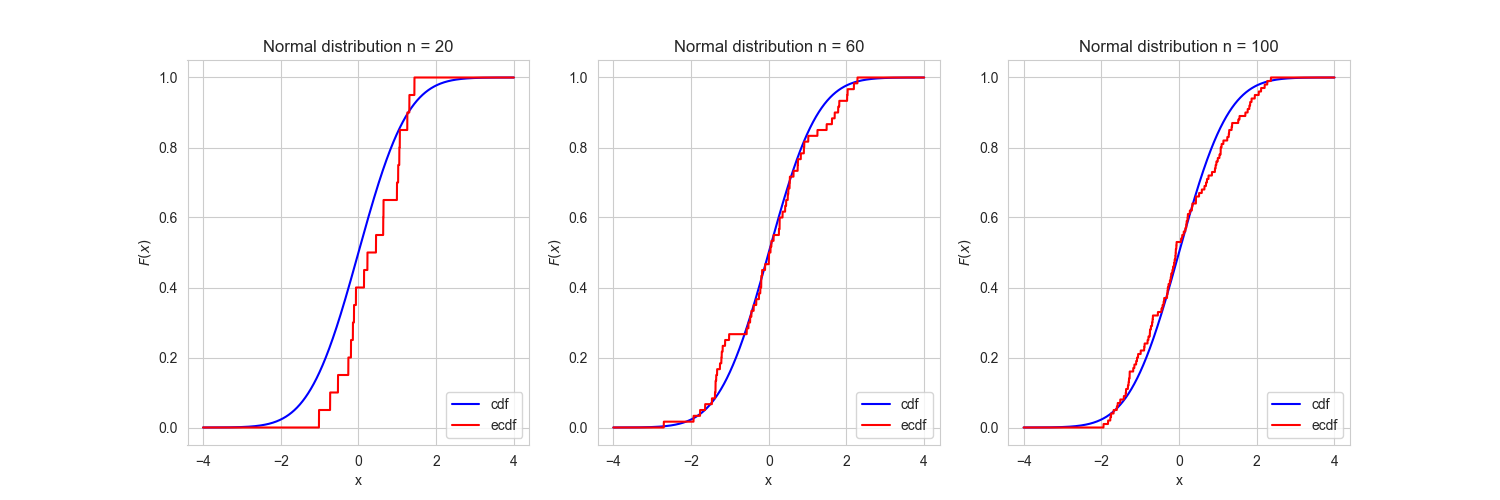
\includegraphics[scale=0.48]{./lab1_4/pictures/Normal distribution100.png}
		\caption{Нормальное распределение}
	\end{figure}
	
	\begin{figure}[H]
		\centering
		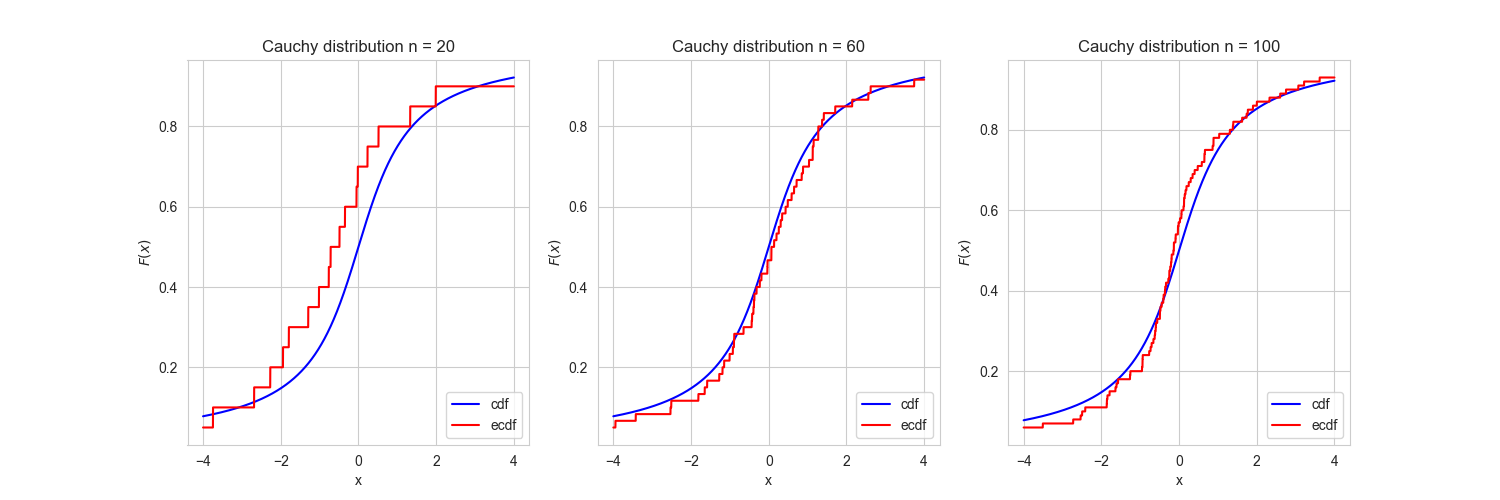
\includegraphics[scale=0.48]{./lab1_4/pictures/Cauchy distribution100.png}
		\caption{Распределение Коши}
	\end{figure}
	
	\begin{figure}[H]
		\centering
		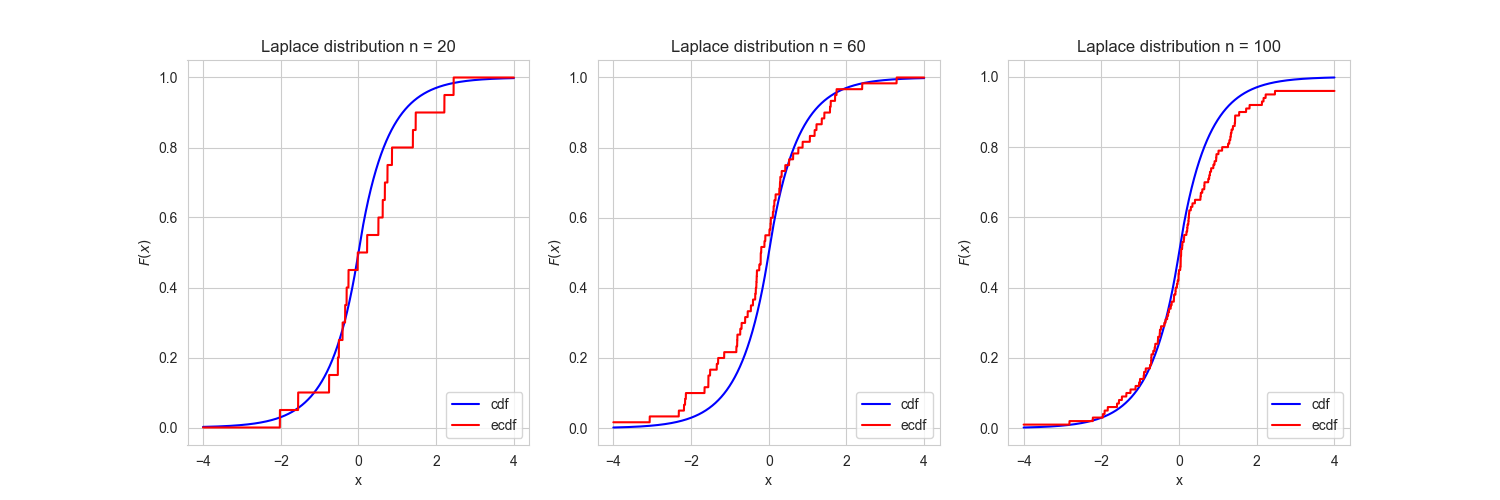
\includegraphics[scale=0.48]{./lab1_4/pictures/Laplace distribution100.png}
		\caption{Распределение Лапласа}
	\end{figure}
	
	\begin{figure}[H]
		\centering
		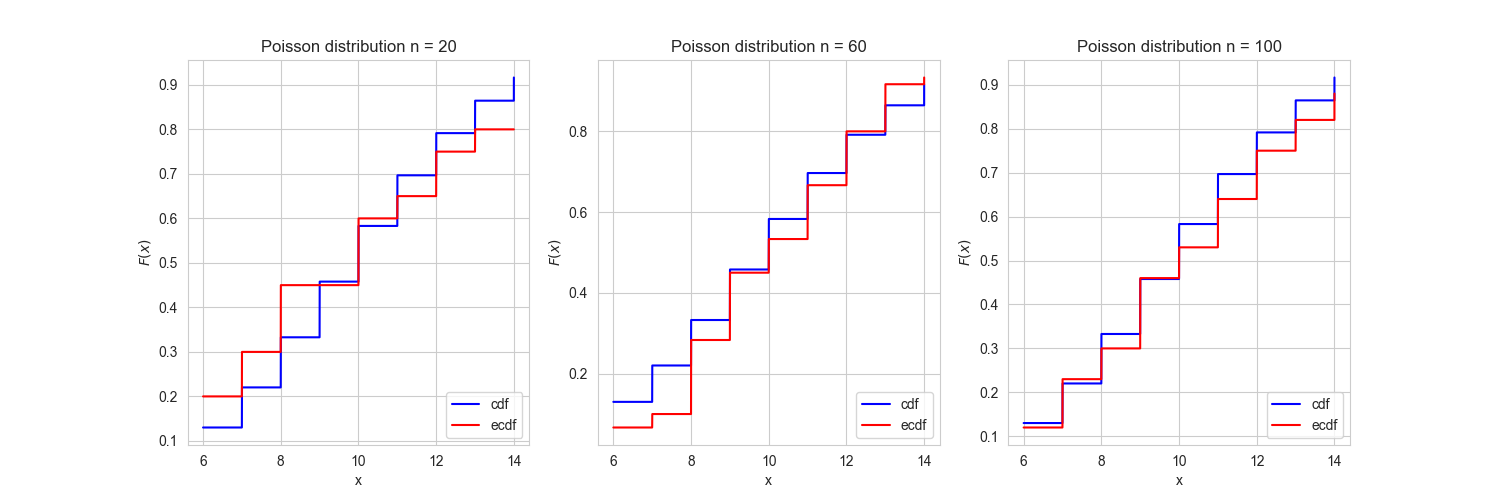
\includegraphics[scale=0.48]{./lab1_4/pictures/Poisson distribution100.png}
		\caption{Распределение Пуассона}
	\end{figure}
	
	\begin{figure}[H]
		\centering
		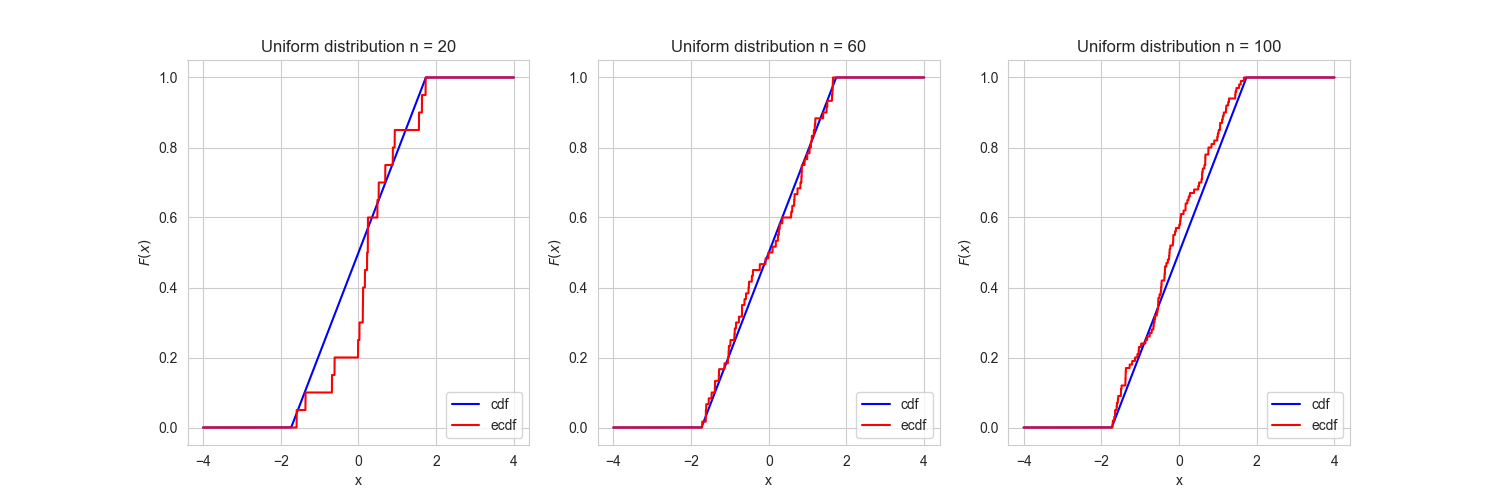
\includegraphics[scale=0.48]{./lab1_4/pictures/Uniform distribution100.png}
		\caption{Равномерное распределение}
	\end{figure}
	\subsection{Ядерные оценки плотности распределения}
	\begin{figure}[H]
		\centering
		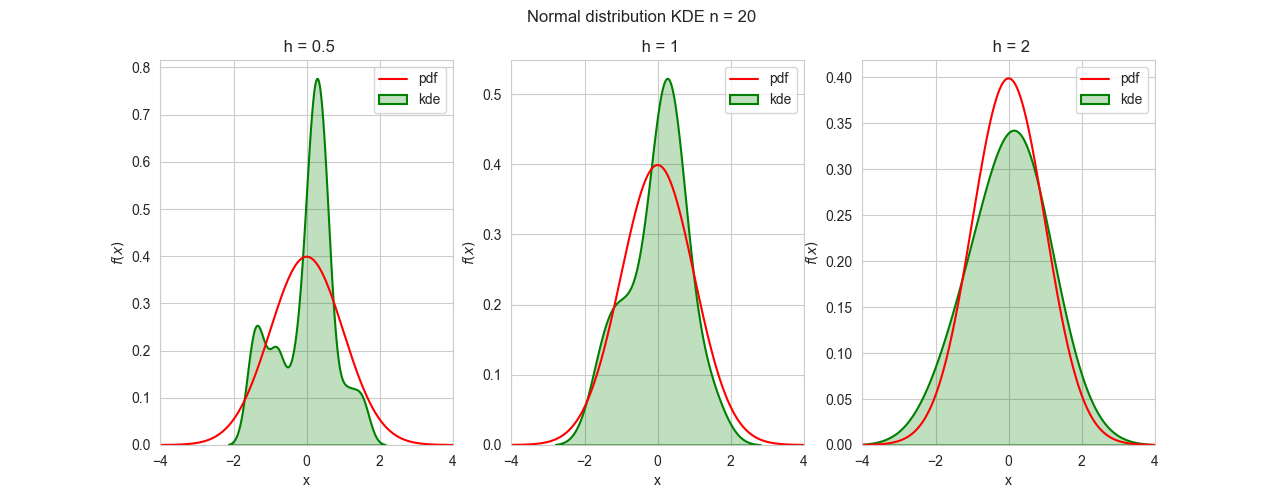
\includegraphics[scale=0.48]{./lab1_4/pictures/Normal distributionKDE20.png}
		\caption{Нормальное распределение размерностью 20}
	\end{figure}
	
	\begin{figure}[H]
		\centering
		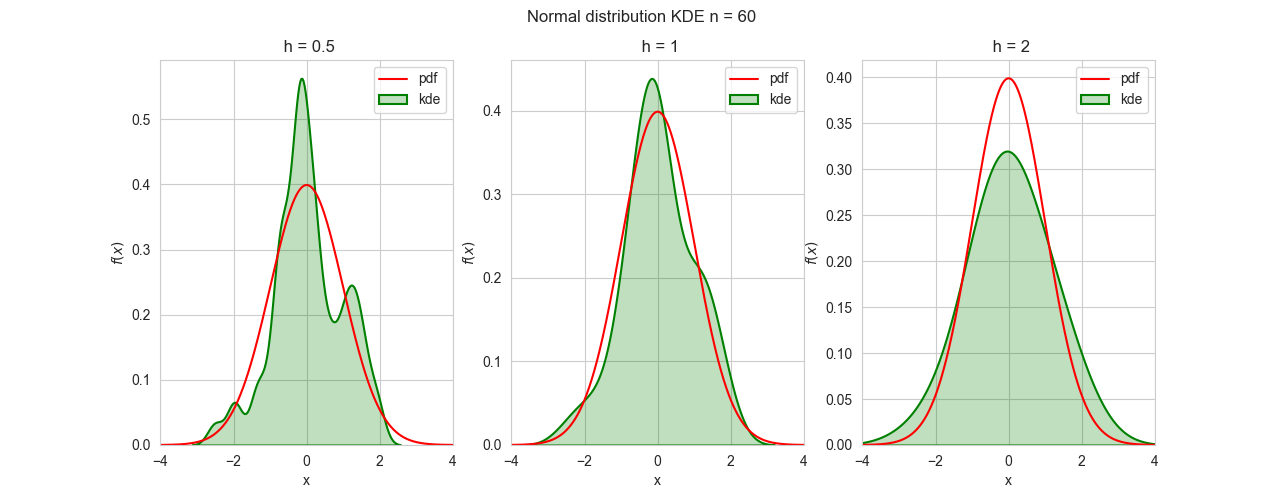
\includegraphics[scale=0.48]{./lab1_4/pictures/Normal distributionKDE60.png}
		\caption{Нормальное распределение размерностью 60}
	\end{figure}
	
	\begin{figure}[H]
		\centering
		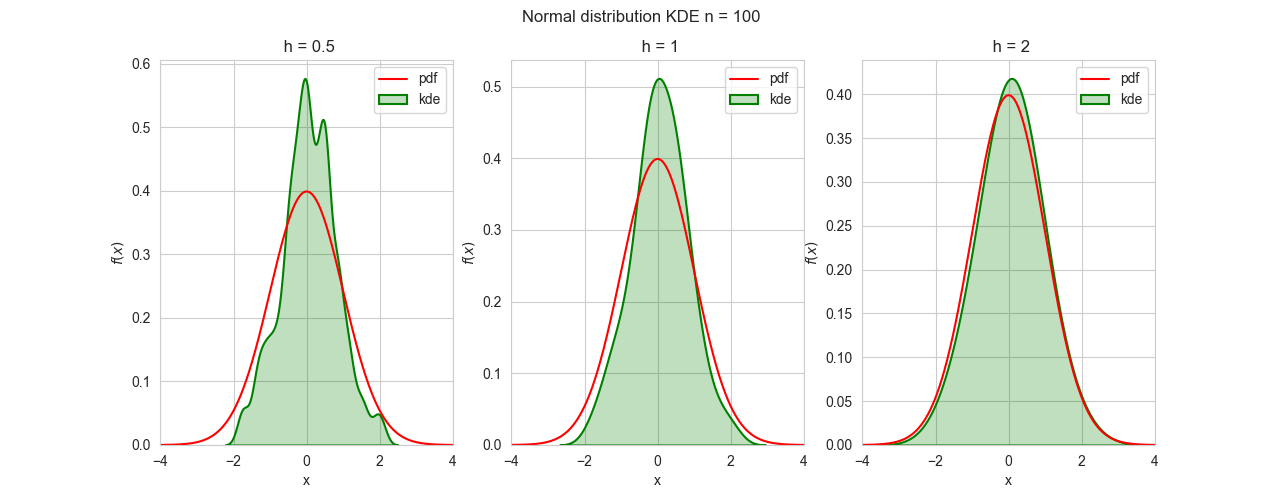
\includegraphics[scale=0.48]{./lab1_4/pictures/Normal distributionKDE100.png}
		\caption{Нормальное распределение размерностью 100}
	\end{figure}
	
	\begin{figure}[H]
		\centering
		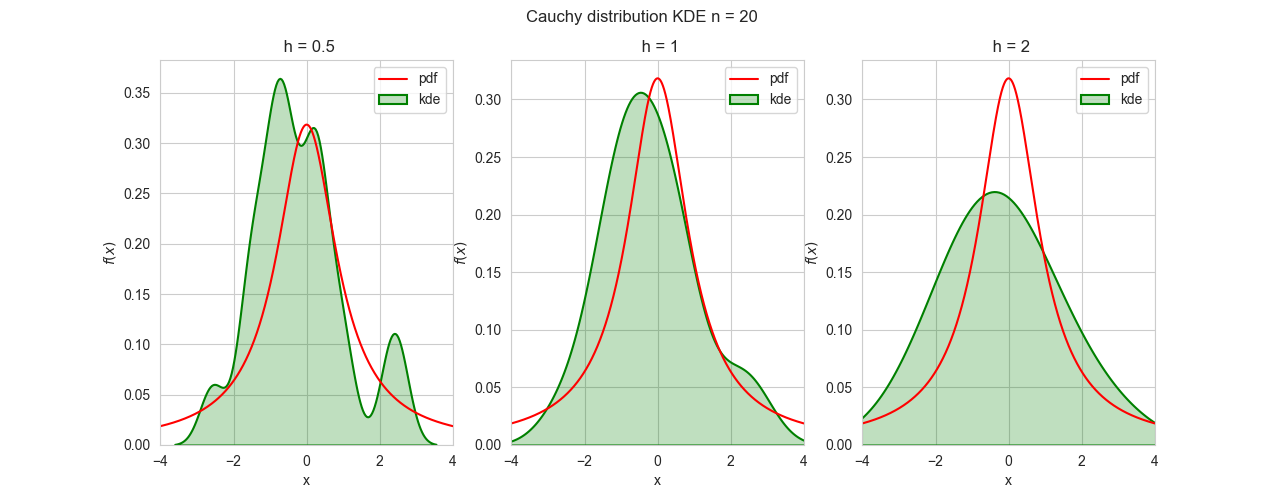
\includegraphics[scale=0.48]{./lab1_4/pictures/Cauchy distributionKDE20.png}
		\caption{Распределение Коши размерностью 20}
	\end{figure}
	
	\begin{figure}[H]
		\centering
		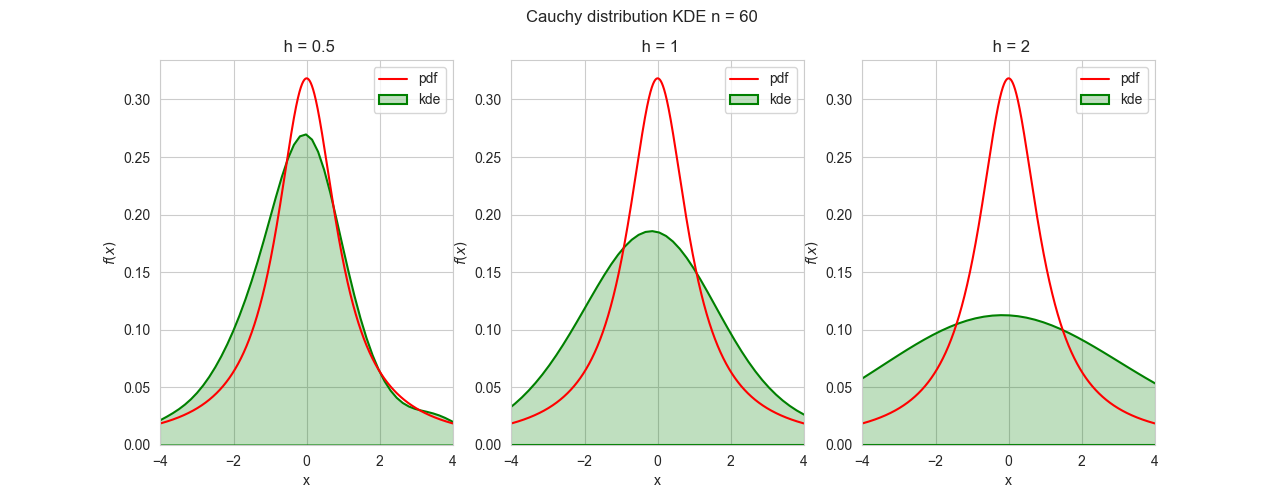
\includegraphics[scale=0.48]{./lab1_4/pictures/Cauchy distributionKDE60.png}
		\caption{Распределение Коши размерностью 60}
	\end{figure}
	
	\begin{figure}[H]
		\centering
		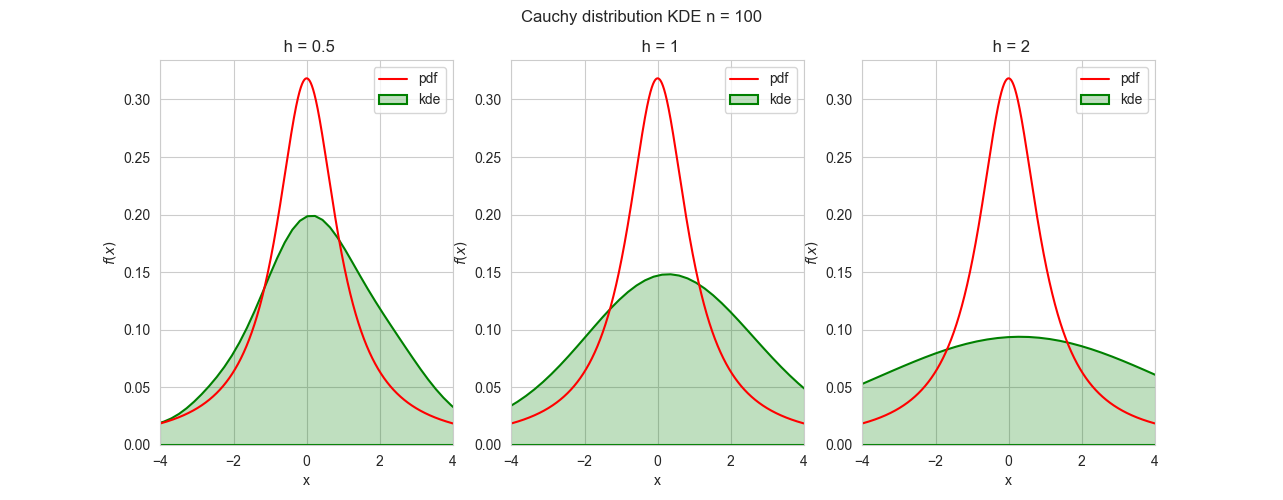
\includegraphics[scale=0.48]{./lab1_4/pictures/Cauchy distributionKDE100.png}
		\caption{Распределение Коши размерностью 100}
	\end{figure}
	
	\begin{figure}[H]
		\centering
		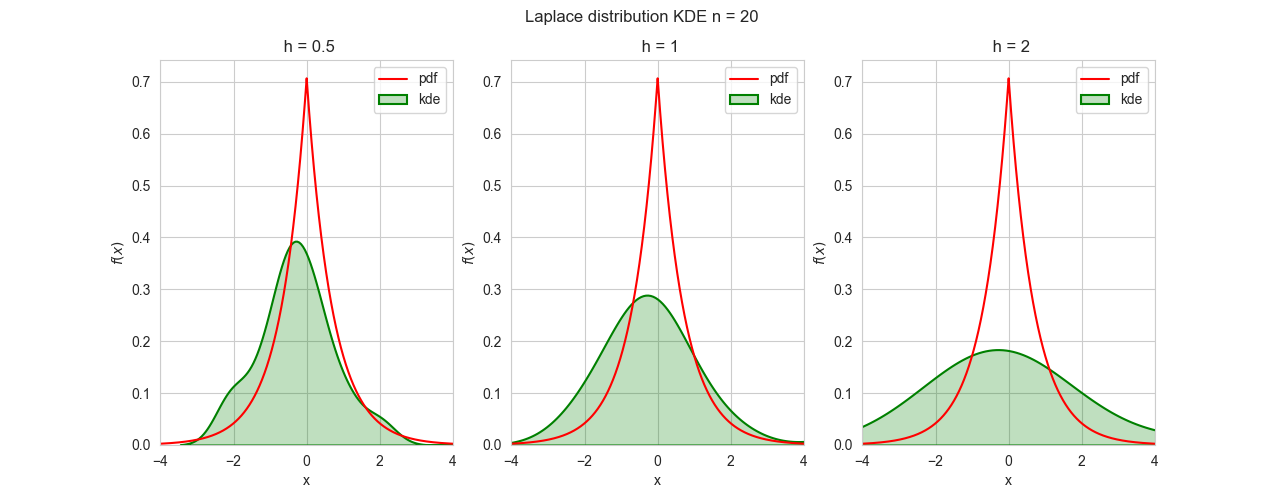
\includegraphics[scale=0.48]{./lab1_4/pictures/Laplace distributionKDE20.png}
		\caption{Распределение Лапласа размерностью 20}
	\end{figure}
	
	\begin{figure}[H]
		\centering
		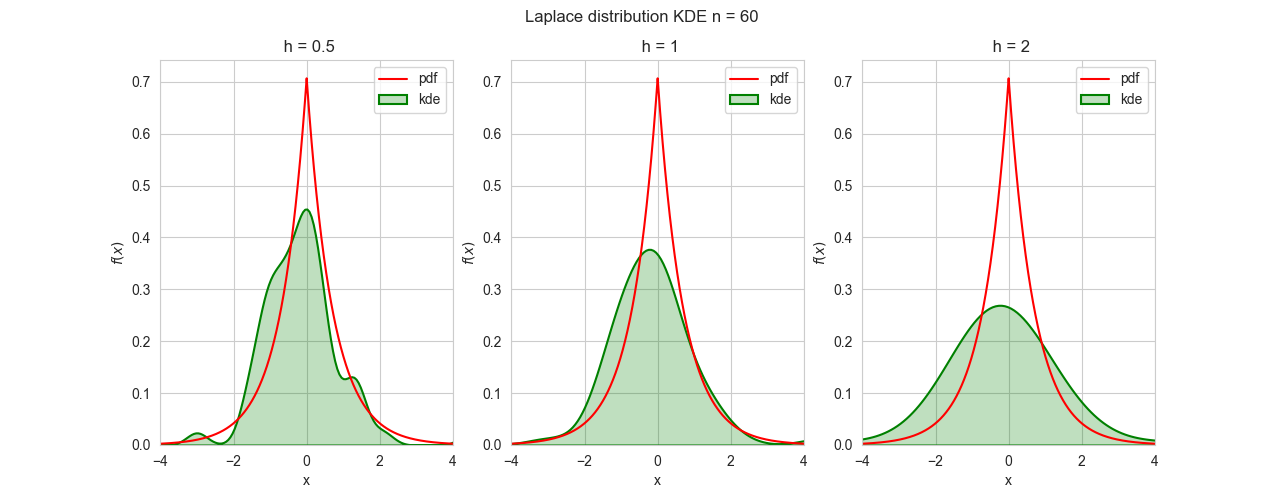
\includegraphics[scale=0.48]{./lab1_4/pictures/Laplace distributionKDE60.png}
		\caption{Распределение Лапласа размерностью 60}
	\end{figure}
	
	\begin{figure}[H]
		\centering
		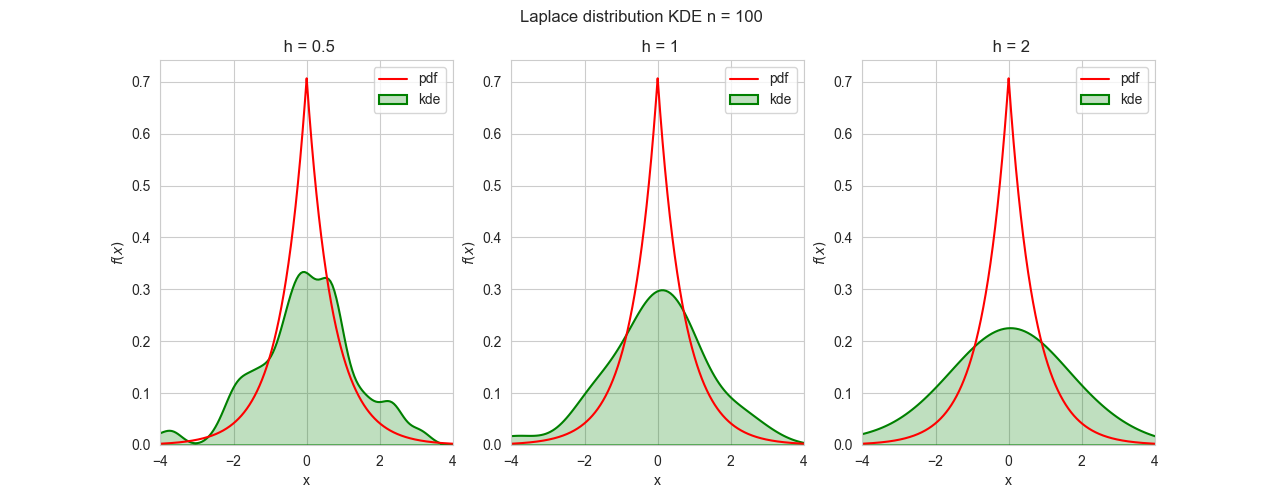
\includegraphics[scale=0.48]{./lab1_4/pictures/Laplace distributionKDE100.png}
		\caption{Распределение Лапласа размерностью 100}
	\end{figure}
	
	\begin{figure}[H]
		\centering
		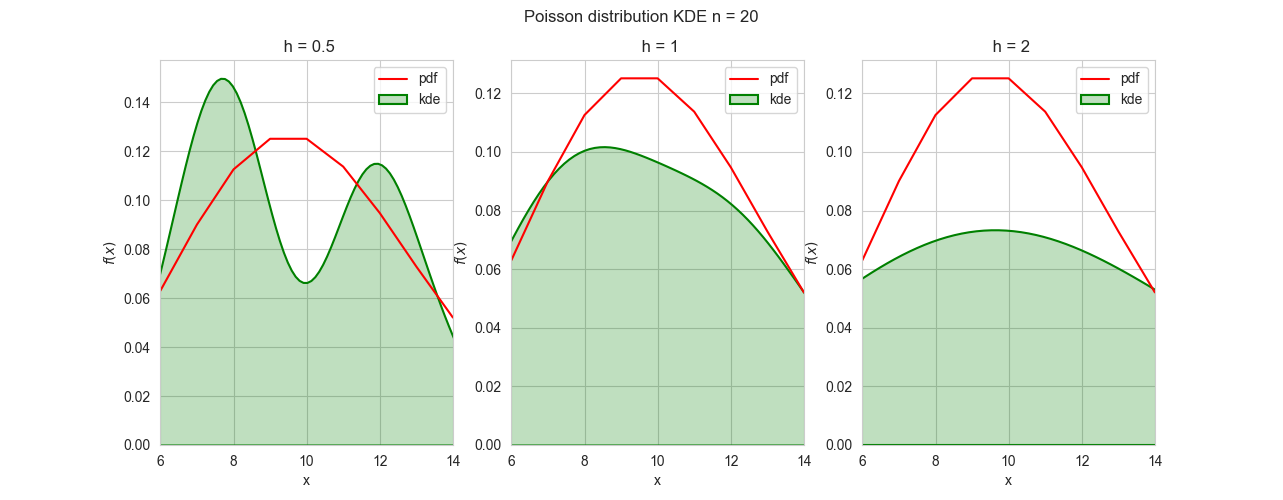
\includegraphics[scale=0.48]{./lab1_4/pictures/Poisson distributionKDE20.png}
		\caption{Распределение Пуассона размерностью 20}
	\end{figure}
	
	\begin{figure}[H]
		\centering
		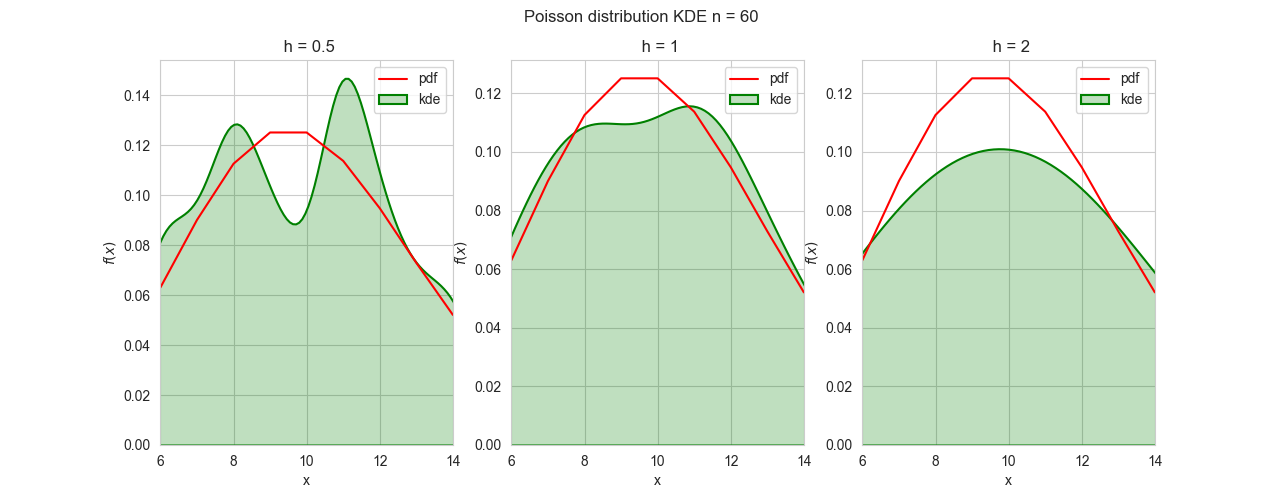
\includegraphics[scale=0.48]{./lab1_4/pictures/Poisson distributionKDE60.png}
		\caption{Распределение Пуассона размерностью 60}
	\end{figure}
	
	\begin{figure}[H]
		\centering
		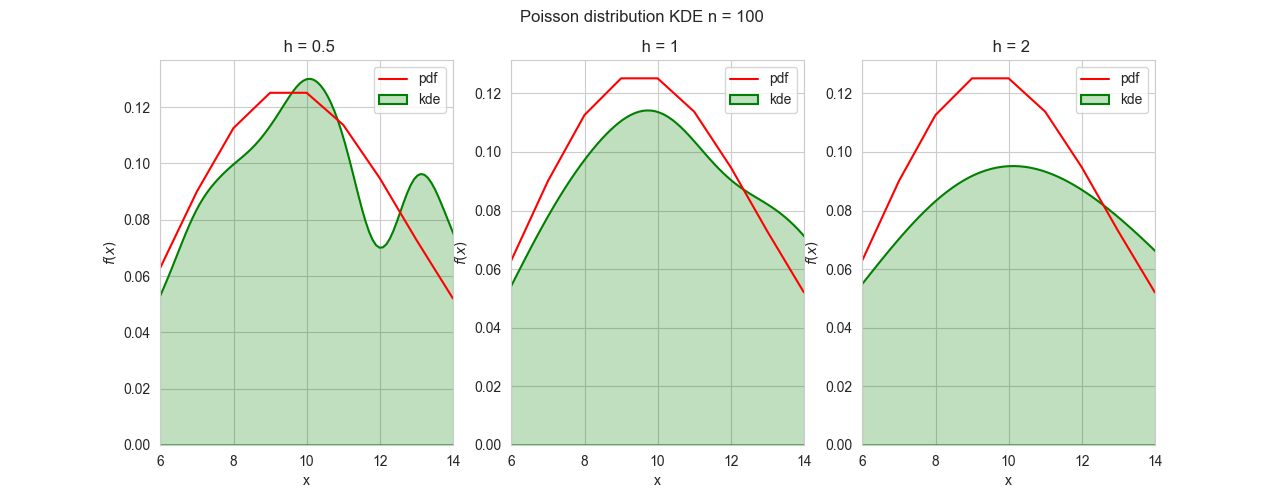
\includegraphics[scale=0.48]{./lab1_4/pictures/Poisson distributionKDE100.png}
		\caption{Распределение Пуассона размерностью 100}
	\end{figure}
	
	\begin{figure}[H]
		\centering
		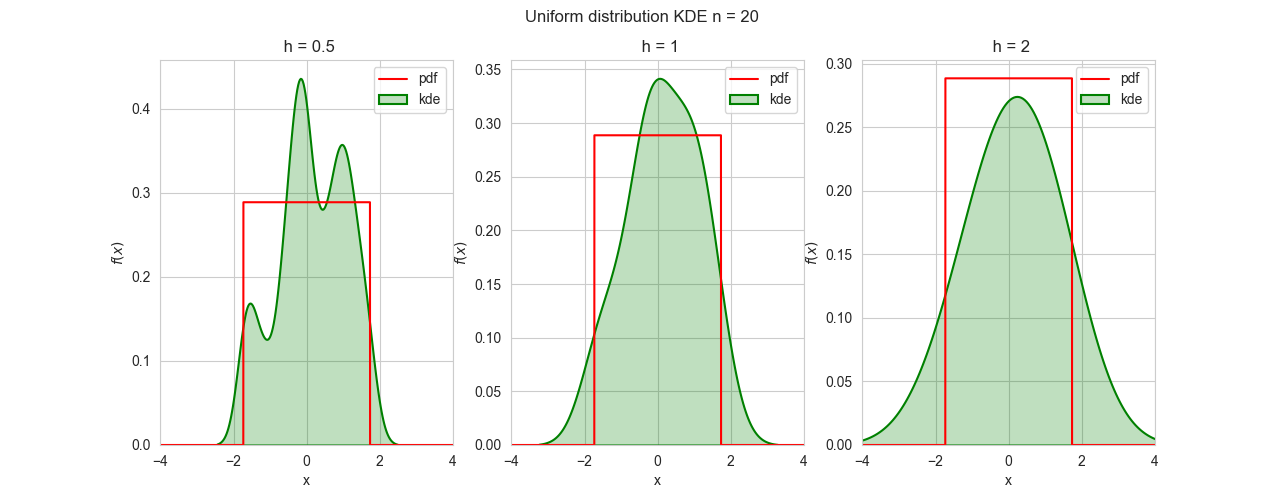
\includegraphics[scale=0.48]{./lab1_4/pictures/Uniform distributionKDE20.png}
		\caption{Равномерное распределение размерностью 20}
	\end{figure}
	
	\begin{figure}[H]
		\centering
		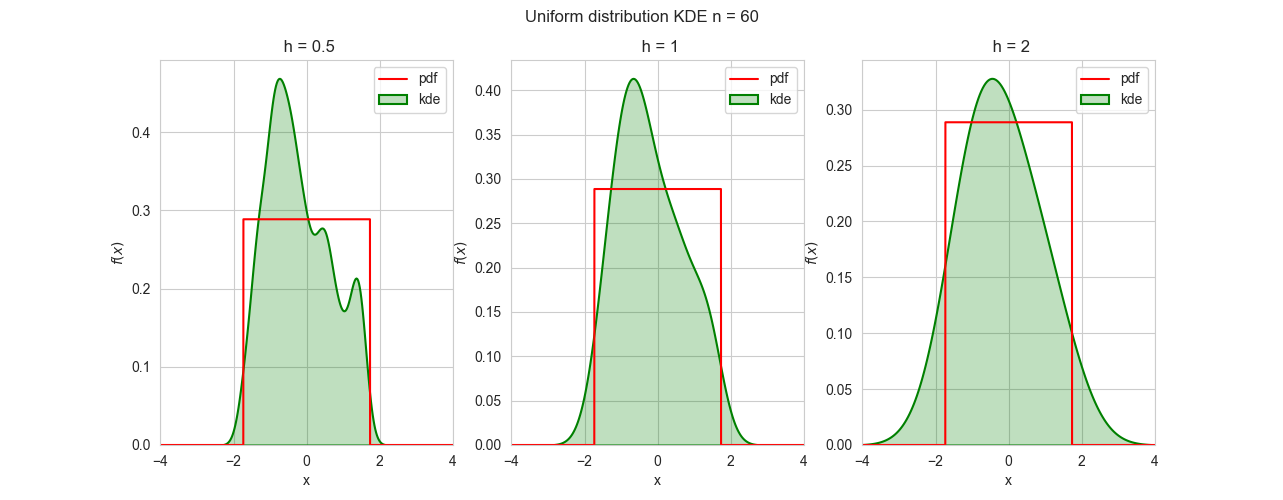
\includegraphics[scale=0.48]{./lab1_4/pictures/Uniform distributionKDE60.png}
		\caption{Равномерное распределение размерностью 60}
	\end{figure}
	
	\begin{figure}[H]
		\centering
		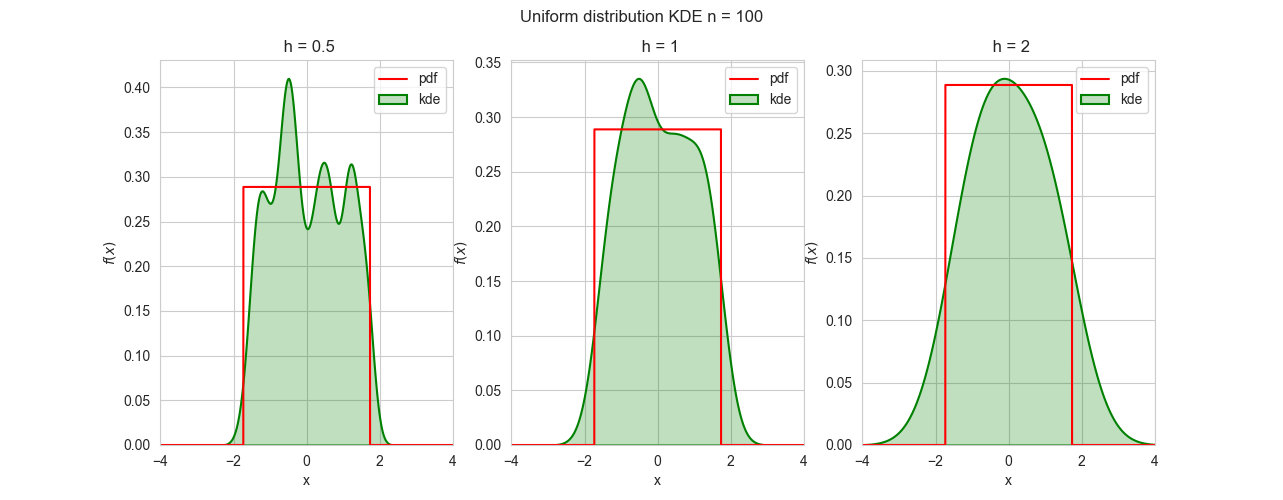
\includegraphics[scale=0.48]{./lab1_4/pictures/Uniform distributionKDE100.png}
		\caption{Равномерное распределение размерностью 100}
	\end{figure}
	\newpage
	\section{Обсуждение}
	\subsection{Гистограмма и график плотности распределения}
	
	По итогам проделанной работы можем сделать вывод о том, что чем
больше выборка для каждого из распределений, тем больше ее гистограмма становится похожей по форме на график плотности вероятности того закона, по которому распределены
величины сгенерированной выборки. 
	~\\
	~\\
	Чем меньше выборка, тем сложнее верно определить характер распределения. Также можно заметить, что максимумы гистограмм и плотностей распределения почти нигде не совпали. Внекоторых местах наблюдаются всплески гистограмм, что наиболее хорошо прослеживается на гистограмме распределения Коши.
	
	
	\subsection{Характеристики положения и рассеяния}
	Исходя из полученных результатов, приведенных в таблицах, можно судить о том, что для нормального распределения, распределения Лапласа, распределения Пуассона и равномерного распределения $D(z)$ для всех характеристик уменьшается с ростом выборки, тогда как $E(z)$ для распределения Пуассона для всех характеристик близко к 10, для остальных трех распределений $E(z)$ уменьшается.	
	~\\
	~\\
	Важно заметить, что дисперсия характеристик рассеяния для распределения Коши является некой аномалией: значения слишком большие даже при увеличении размера выборки. Данное поведение можно обосновать наличием различных выбросов, бесконечностью дисперсии случайной величины и неопределенностью математического ожидания распределенной по данному закону.
	
	\subsection{Боксплот Тьюки, доля и теоретическая вероятность выбросов}
	Бокспот Тьюки позволяет наглядно оценивать важные характеристики распределений. Так, исходя из полученных рисунков, видно то, что мы трудоёмко анализировали в предыдущих частях.
		~\\
	~\\
		По данным, приведенным в таблице, можно сказать, что чем больше выборка, тем ближе доля выбросов будет к теоретической оценке. 
		~\\
	~\\
	Для распределения Коши доля выбросов значительно выше, чем для остальных
распределений. Равномерное распределение же в точности повторяет теоретическую оценку - выбросов мы не получали.
	
	\subsection{Эмпирическая функция и ядерные оценки плотности распределения}
	
	Проанализировав графики эмпирических функций, можно сделать выводы, что чем больше берется размерность выборки, тем ближе функция распределения реальной выборки к ступенчатой эмпирической функции распределения. Заметим также, что для распределения Пуассона и равномерного распределения отклонение функций друг от друга наибольшее.
~\\
	~\\
Графики ядерных оценок показывают, что чем больше размер выборки, тем ближе ядерные оценки и функции плотности вероятности для всех $h$. Для распределения Пуассона наиболее ярко видно, как сглаживает отклонения увеличение параметра сглаживания $h$.
~\\
~\\
В зависимости от особенностей распределений для их описания в ядерной оценке лучше подходят разные параметры $h$. Для равномерного распределения и распределения Пуассона лучше подойдет параметр $h= 2h_n$, для распределения Лапласа - $h = h_n/2$, а для нормального и Коши - $h = h_n$. 


	\newpage
\addcontentsline{toc}{section}{Литература}

\begin{thebibliography}{4}
    \bibitem{s:hist}
    Histogram. URL: \url{https://en.wikipedia.org/wiki/Histogram}
    \bibitem{b:probSectMath}
    Вероятностные разделы математики. Учебник для бакалавров технических направлений.//Под ред. Максимова Ю.Д. --- Спб.: «Иван Федоров», 2001. --- 592 c., илл.
    \bibitem{s:boxplot}
    Box plot. URL: \url{https://en.wikipedia.org/wiki/Box_plot}
    \bibitem{a:nonParamRegr}
    Анатольев, Станислав (2009) «Непараметрическая регрессия», Квантиль, №7, стр. 37-52.
\end{thebibliography}


\end{document}